\section{Results and Analysis}
\label{sec:results}
\subsection{Candidate access and displacement}
Table~\ref{tab:coverage} counts query--drug candidate records and covered positive pairs in both cohorts. The union expands positive access, but most graph candidates are not evidence members. In replay, shared membership accounts for only 120/1,580 candidate records yet contains 19/33 covered positives. The 318 evidence-exclusive records add 13 positives; the 1,142 graph-exclusive records add one.
% Generated from frozen artifacts; edit build_revision_tables.py, not numeric cells.
\begin{table}[t]
\centering
\caption{Candidate coverage}
\label{tab:coverage}
\small
\setlength{\tabcolsep}{4pt}
\begin{tabular}{lrrrr}
\toprule
Support & Dev. records & Dev. pairs & Replay records & Replay pairs \\
\midrule
Graph $R_0$ & 874 & 19/43 & 1,262 & 20/46 \\
Evidence $E$ & 360 & 23/43 & 438 & 32/46 \\
Union $R_1$ & 1,051 & 24/43 & 1,580 & 33/46 \\
Shared $R_0\cap E$ & 183 & 18/43 & 120 & 19/46 \\
Graph only & 691 & 1/43 & 1,142 & 1/46 \\
Evidence only & 177 & 5/43 & 318 & 13/46 \\
\bottomrule
\end{tabular}
\end{table}


Wider access does not ensure better placement. Replay Mix loses 0.0093 query MRR relative to Graph despite raising pair coverage from 20/46 to 33/46. Equation~\eqref{eq:decomposition} attributes this change to original-positive displacement of $-0.0310$ and a newly accessible-positive increment of $+0.0217$. The same SF scores are used before and after expansion. Thus displacement reflects insertion of additions ahead of old positives, not model refitting or a score change.

Development shows the same distinction at a larger magnitude: Mix loses 0.0641 MRR, comprising $-0.1395$ displacement and $+0.0754$ access gain. Append-SF fixes old absolute positions and gains 0.0737 over Graph. Its replay gain is smaller, $+0.0102$ (Table~\ref{tab:main}).

\subsection{Same-pool controls and retrieval depth}
% Generated from frozen artifacts; edit build_revision_tables.py, not numeric cells.
\begin{table}[t]
\centering
\caption{Main results}
\label{tab:main}
\small
\setlength{\tabcolsep}{3pt}
\begin{tabular}{lrrrrrr}
\toprule
Method & Pair cov. & MRR$_q$ & MRR$_p$ & HR@1 & HR@3 & HR@5 \\
\midrule
\multicolumn{7}{l}{\textit{January development: 41 queries, 43 pairs}} \\
Graph & 19/43 & 0.2996 & 0.2857 & 9/41 & 15/41 & 15/41 \\
Mix & 24/43 & 0.2355 & 0.2252 & 6/41 & 12/41 & 16/41 \\
CIViC branch & 23/43 & 0.3660 & 0.3490 & 10/41 & 20/41 & 21/41 \\
Append-SF & 24/43 & 0.3733 & 0.3565 & 12/41 & 18/41 & 18/41 \\
AltGraph & 19/43 & 0.3409 & 0.3250 & 12/41 & 15/41 & 15/41 \\
AltAppend & 24/43 & 0.4146 & 0.3959 & 15/41 & 18/41 & 18/41 \\
Borda & 24/43 & 0.4621 & 0.4411 & 17/41 & 21/41 & 22/41 \\
Context & 24/43 & 0.3660 & 0.3496 & 10/41 & 20/41 & 21/41 \\
Shared-first & 24/43 & 0.3750 & 0.3581 & 10/41 & 20/41 & 22/41 \\
RRF & 24/43 & 0.4594 & 0.4386 & 17/41 & 20/41 & 22/41 \\
\midrule
\multicolumn{7}{l}{\textit{Retrospective new-context replay: 45 queries, 46 pairs}} \\
Graph & 20/46 & 0.1902 & 0.1860 & 7/45 & 9/45 & 10/45 \\
Mix & 33/46 & 0.1809 & 0.1774 & 6/45 & 8/45 & 9/45 \\
CIViC branch & 32/46 & 0.3452 & 0.3386 & 7/45 & 23/45 & 27/45 \\
Append-SF & 33/46 & 0.2004 & 0.1965 & 7/45 & 9/45 & 10/45 \\
AltGraph & 20/46 & 0.1227 & 0.1201 & 2/45 & 4/45 & 11/45 \\
AltAppend & 33/46 & 0.1330 & 0.1305 & 2/45 & 4/45 & 11/45 \\
Borda & 33/46 & 0.3040 & 0.2979 & 9/45 & 14/45 & 16/45 \\
Context & 33/46 & 0.3460 & 0.3389 & 7/45 & 23/45 & 27/45 \\
Shared-first & 33/46 & 0.4265 & 0.4176 & 13/45 & 24/45 & 27/45 \\
RRF & 33/46 & 0.3895 & 0.3816 & 11/45 & 21/45 & 27/45 \\
\bottomrule
\end{tabular}
\end{table}

RRF improves replay MRR over Append-SF by 0.1891 and AltAppend by 0.2566. The stronger same-pool comparison is smaller: RRF reaches 0.3895 versus 0.3460 for Context, a difference of $+0.0435$. Both drug- and source-component 95\% intervals span zero (Table~\ref{tab:paired}). RRF improves nine query-best ranks, worsens 13 and ties 23; the reciprocal-rank magnitudes give a positive mean despite more losses. Across the 43 leave-one-component analyses, its Context difference remains positive, ranging from $+0.0097$ to $+0.0802$. This omission result does not override the bootstrap uncertainty.
% Generated from frozen artifacts; edit build_revision_tables.py, not numeric cells.
\begin{table}[t]
\centering
\caption{Paired replay comparisons}
\label{tab:paired}
\small
\setlength{\tabcolsep}{2.5pt}
\begin{tabular}{lrrrr}
\toprule
Comparison & $\Delta$MRR & Drug 95\% interval & Source 95\% interval & W/T/L \\
\midrule
RRF--Context & +0.0435 & $[\,-0.0692,\,+0.1718\,]$ & $[\,-0.0652,\,+0.1666\,]$ & 9/23/13 \\
RRF--CIViC & +0.0444 & $[\,-0.0683,\,+0.1732\,]$ & $[\,-0.0639,\,+0.1670\,]$ & 10/23/12 \\
Shared--Context & +0.0805 & $[\,-0.0237,\,+0.2034\,]$ & $[\,-0.0210,\,+0.2046\,]$ & 11/31/3 \\
RRF--Shared & -0.0369 & $[\,-0.1624,\,+0.1061\,]$ & $[\,-0.1608,\,+0.1029\,]$ & 6/25/14 \\
\bottomrule
\end{tabular}
\end{table}


\paragraph{Shared membership.}
A simple shared-first control reproduces and exceeds RRF's observed replay MRR gain over Context. Placing shared candidates first in the complete Context order raises replay MRR from 0.3460 to 0.4265, a gain of $+0.0805$. Shared denotes this Shared-first Context control in Table~\ref{tab:paired}. Moving from that control to RRF changes MRR by $-0.0369$. Both stepwise comparisons have paired intervals spanning zero. Development reverses the ordering: RRF reaches 0.4594 versus 0.3750 for Shared-first. These two steps isolate specified ranking changes, not causal fractions of graph and clinical information, and do not select a new default.

\paragraph{Depth and positive retention.}
Shared-first, RRF and Context all hit 27/45 replay queries at five, while their rank-one hits are 13, 11 and seven, and rank-three hits are 24, 21 and 23 (Fig.~\ref{fig:hrk}). Context and CIViC coincide at the plotted cutoffs; their distinct markers identify both policies. Pair-level outcomes also differ. Context places 11/13 evidence-exclusive positives in the top five, versus nine for Shared-first and eight for RRF. Of the ten positives already in Append-SF's top five, the respective policies retain seven, nine and ten. These pair counts are distinct from query HR.
\begin{figure}[t]
\centering
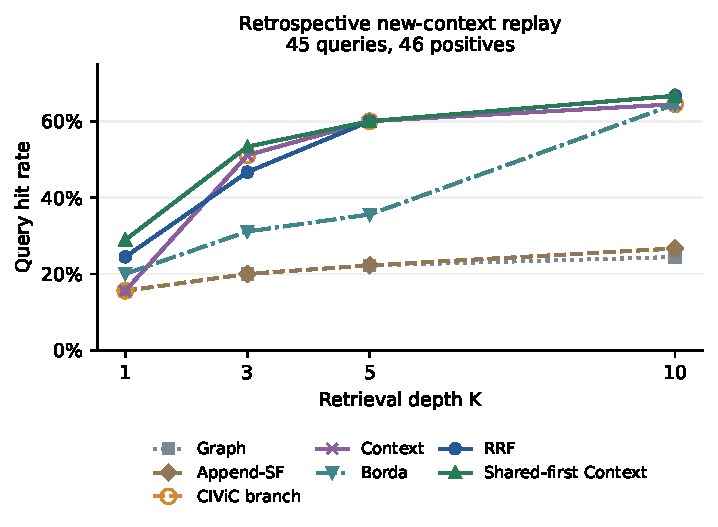
\includegraphics[width=.96\textwidth]{generated/replay_hr_at_k_with_context.pdf}
\caption{Hit rates}
\label{fig:hrk}
\end{figure}


The CIViC-only comparison changes support as well as order. Its replay MRR is 0.3452, with 27/45 hits at five. The single extra covered positive under RRF is dasatinib for MP:6050 at rank 28; it contributes at most $1/(45\cdot28)=0.0008$ query MRR. Most of the $+0.0444$ difference therefore concerns already accessible positives, but the paired intervals still span zero.

\paragraph{Conditional source order.}
Table~\ref{tab:order-ablation} adds graph-order permutations to the archived clinical-order experiment. Replay graph shuffling lowers mean MRR by 0.0462 and HR@3 by 9.07 percentage points. Its MRR upper-tail $p=0.0324$ becomes 0.2915 after the specified 12-test Holm correction. Clinical shuffling lowers mean replay HR@5 by 9.15 points; 17/5,000 draws match or exceed the observed 27 hits, giving $p=18/5001=0.0036$ and Holm $p=0.0432$. Only that comparison survives 0.05 across the family. Development graph MRR exceeds its central 95\% upper quantile, but its Holm $p=0.0550$.
% Generated from frozen artifacts; edit build_revision_tables.py, not numeric cells.
\begin{table}[t]
\centering
\caption{Order shuffles}
\label{tab:order-ablation}
\small
\setlength{\tabcolsep}{2.2pt}
\begin{tabular}{llrrrrr}
\toprule
Shuffled & Metric & Observed & Mean & Central 95\% & Upper $p$ & Holm $p$ \\
\midrule
Graph & MRR & 0.3895 & 0.3433 & $[\,0.2974,\,0.3929\,]$ & 0.0324 & 0.2915 \\
Graph & HR@3 (\%) & 46.67 & 37.59 & $[\,31.11,\,44.44\,]$ & 0.0074 & 0.0740 \\
Graph & HR@5 (\%) & 60.00 & 57.07 & $[\,53.33,\,60.00\,]$ & 0.2044 & 1.0000 \\
CIViC & MRR & 0.3895 & 0.3514 & $[\,0.3085,\,0.3969\,]$ & 0.0498 & 0.3983 \\
CIViC & HR@3 (\%) & 46.67 & 42.82 & $[\,35.56,\,48.89\,]$ & 0.2134 & 1.0000 \\
CIViC & HR@5 (\%) & 60.00 & 50.85 & $[\,46.67,\,55.56\,]$ & 0.0036 & 0.0432 \\
\bottomrule
\end{tabular}
\end{table}


Membership and the unshuffled branch's complete order remain fixed, including the clinical SF terminal key. Accordingly, these perturbations quantify conditional order sensitivity, not removal of all information from either source. The replay graph lists have median length 30 (range 0--50; one empty), and clinical lists median eight (0--36; two empty). Empty branches remain in the denominator; full distributions and all 12 comparisons are retained in S1.

\subsection{Limits under two fixed source orders}
\begin{table}[t]
\caption{Interleaving results}
\label{tab:oracle}
\centering\small
\begin{tabularx}{\textwidth}{@{}l@{\hspace{6pt}}X@{\hspace{5pt}}r@{}}
\toprule
Policy & Ordering constraint & MRR$_q$ \\
\midrule
Append-SF & $O$ followed by $N_{\mathrm{SF}}$ & 0.2004 \\
Append-CIViC & $O$ followed by $N_e$ & 0.2018 \\
Original insertion & Fixed $O,N_v$, $\lambda=4$ & 0.2064 \\
Evidence insertion & Fixed $O,N_e$, $\lambda=4$ & 0.2065 \\
Two-sequence oracle & Best merge of $O,N_e$ & 0.3294 \\
RRF & Full $L_g,L_e$ fusion & 0.3895 \\
Old-order oracle & Fixed $O$, freely ordered additions & 0.4568 \\
\bottomrule
\end{tabularx}
\end{table}
Changing the append suffix from SF to CIViC order barely changes MRR; both yield ten top-five hits (Table~\ref{tab:oracle}). The two insertion policies also yield ten hits. At the development-selected penalty, both retain all old top-five positives and place none of the 13 evidence-exclusive positives in the top five.

The best label-informed merge of fixed $O,N_e$ reaches at most 0.3294 MRR under Eq.~\eqref{eq:bound}, below RRF's 0.3895. These label-informed oracles are explanatory ceilings, not deployable rankings. Exceeding the two-sequence ceiling implies relaxing at least one of the two specified within-sequence constraints. It does not imply that the graph order must change: preserving only that order and freely reordering additions raises the ceiling to 0.4568.

% Generated from frozen artifacts; edit build_revision_tables.py, not numeric cells.
\begin{table}[t]
\centering
\caption{Case study}
\label{tab:cases}
\small
\setlength{\tabcolsep}{2pt}
\begin{tabular}{llrrrrr}
\toprule
Query context & Drug & App. & Alt. & Ctx. & Shared & RRF \\
\midrule
Jan. Breast MP:263 & dovitinib & 41 & 41 & 1 & 4 & 5 \\
Jan. Breast MP:263 & erdafitinib & 33 & 6 & 40 & 40 & 41 \\
W1 Colorectal MP:5117 & pembrolizumab & 7 & 7 & 1 & 1 & 2 \\
W1 Midline glioma MP:3807 & dordaviprone & 14 & 14 & 1 & 1 & 1 \\
W3 Melanoma MP:281$^*$ & belvarafenib & -- & -- & -- & -- & -- \\
\bottomrule
\end{tabular}
\end{table}

The original five case-study rows are retained with the new controls (Table~\ref{tab:cases}), where App., Alt., Ctx. and Shared denote Append-SF, AltAppend, Context and Shared-first Context. A dash marks an unretrieved positive; the asterisk identifies cutoff-defined belvarafenib, outside the 45-query replay. For January breast MP:263, RRF moves evidence-exclusive dovitinib from rank 41 under Append-SF to five, while Context already puts it first. Graph-exclusive erdafitinib moves from 33 to 41 under RRF. In replay, Context and Shared-first already place pembrolizumab and dordaviprone first; fusion is not required for those successes. The unretrieved cutoff-defined belvarafenib remains a negative case.

Provenance describes the cross-context links without validating treatment efficacy. Of 27 RRF top-five replay positives, 13 have cutoff benefit evidence for the exact profile in another or unspecified disease, while 14 share a gene with the evidence profile. For example, level-B dordaviprone evidence for glioma MP:2289 links to MP:3807 through H3-3A.

\subsection{Dependence and parameter sensitivity}
\label{sec:rq4}
The earlier development RRF--AltAppend analysis uses 17 drug and 18 source components, with $+0.0448$ MRR and intervals $[+0.0102,+0.1099]$ and $[+0.0108,+0.1095]$ (S1). It concerns a different cohort and weaker comparator than the replay Context comparison. Removing development's 14 entrectinib pairs leaves 27 queries and 29 pairs: RRF reaches 0.2142, Append-SF 0.1772 and AltAppend 0.1658; Context can exceed RRF on that subset.

Across 54 fusion settings, RRF's replay MRR always exceeds Append-SF's but improves on Context in only part of the grid. The settings vary $k\in\{10,20,40,60,80,100\}$ and graph weight $\alpha\in\{.1,.2,\ldots,.9\}$. All exceed both Context and CIViC on development MRR. In replay, only 30/54 exceed either strong baseline and 24 fall below; no MRR ties occur. HR@5 has 24 settings above, six tied and 24 below both baselines. In the nine-setting neighborhood $k\in\{40,60,80\}$, $\alpha\in\{.4,.5,.6\}$, replay hits range from 19 to 30 of 45. Thus the all-setting advantage over Append-SF does not establish robustness against stronger baselines; the default remains frozen.

\subsection{Source sensitivity and temporal scope}
% Generated from frozen artifacts; edit build_revision_tables.py, not numeric cells.
\begin{table}[t]
\centering
\caption{Source exclusion}
\label{tab:source-exclusion}
\small
\setlength{\tabcolsep}{3.5pt}
\begin{tabular}{lrrrrr}
\toprule
Policy & MRR$_q$ & Pair cov. & HR@1 & HR@3 & HR@5 \\
\midrule
RRF & 0.3330 & 26/39 & 7/39 & 16/39 & 22/39 \\
Context & 0.2924 & 26/39 & 3/39 & 19/39 & 23/39 \\
CIViC & 0.2915 & 25/39 & 3/39 & 19/39 & 23/39 \\
\bottomrule
\end{tabular}
\end{table}

Linking the evidence actually used at cutoff to frozen label supports identifies overlap for 7/46 replay pairs (15.22\%), affecting six queries. The audit covers 11,171 used-evidence rows and 46 eligible positive-label support rows, with no missing source IDs. These are used-evidence intersections, not occurrences anywhere in the snapshot or only among successful hits.

Removing those labels leaves 39 queries and 39 pairs at unchanged ranks (Table~\ref{tab:source-exclusion}). RRF retains MRR differences of $+0.0406$ from Context and $+0.0415$ from CIViC, but hits one fewer query at five than either. This is descriptive sensitivity: the same publication may support distinct contexts, and neither overlap nor its removal resolves every form of leakage or dependence.

The union covers 14/17, 6/6 and 13/23 replay pairs in W1--W3. It misses 13/46 overall, including ten in W3; no union-ranking policy can retrieve those missing pairs. In the separate three-query cutoff-defined cohort, RRF ranks W1 selpercatinib first and misses both W3 belvarafenib positives. The sealed September--October pilot contains two eligible positives and zero hard cases, below its prespecified minima of ten and three; both positives are unretrieved. These small counts and the retrospective main query construction do not establish prospective generalization.
